% Reflection of a walk path after its first visit to level r. Generated by a short script.
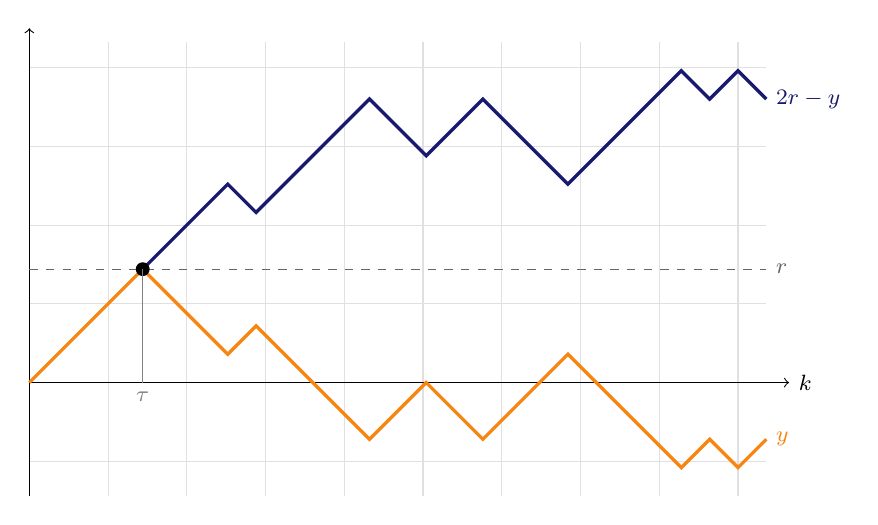
\begin{tikzpicture}[x=0.36cm,y=0.36cm]
\draw[black!12] (0,-4) grid (26,12);
\draw[->] (0,0)--(26.8,0) node[right,font=\footnotesize] {$k$};
\draw[->] (0,-4)--(0,12.5);
\draw[dashed,black!60] (0,4)--(26,4) node[right,font=\footnotesize] {$r$};
\draw[MidnightBlue,very thick] (4,4)--(5,5)--(6,6)--(7,7)--(8,6)--(9,7)--(10,8)--(11,9)--(12,10)--(13,9)--(14,8)--(15,9)--(16,10)--(17,9)--(18,8)--(19,7)--(20,8)--(21,9)--(22,10)--(23,11)--(24,10)--(25,11)--(26,10);
\draw[BurntOrange,very thick] (0,0)--(1,1)--(2,2)--(3,3)--(4,4)--(5,3)--(6,2)--(7,1)--(8,2)--(9,1)--(10,0)--(11,-1)--(12,-2)--(13,-1)--(14,0)--(15,-1)--(16,-2)--(17,-1)--(18,0)--(19,1)--(20,0)--(21,-1)--(22,-2)--(23,-3)--(24,-2)--(25,-3)--(26,-2);
\fill[black] (4,4) circle (2.5pt);
\draw[black!50] (4,4)--(4,0) node[below,font=\footnotesize] {$\tau$};
\node[right,font=\footnotesize,BurntOrange] at (26,-2) {$y$};
\node[right,font=\footnotesize,MidnightBlue] at (26,10) {$2r-y$};
\end{tikzpicture}
